\documentclass[a4paper,12pt]{article}
\linespread{1.3}
\usepackage[left=3cm,top=2cm,right=3cm,bottom=2cm]{geometry}

%\usepackage{palatino}

\usepackage{xypic}
\usepackage{natbib}
\bibliographystyle{plainnat}
\bibpunct{[}{]}{;}{s}{,}{,}

\usepackage[header,page,titletoc]{appendix}
\renewcommand{\appendixname}{Appendix}
%\renewcommand{\appendixtocname}{List of appendices}

\usepackage[colorlinks=true,linkcolor=black,citecolor=black,filecolor=black,menucolor=black,urlcolor=black]{hyperref}
\usepackage{graphicx}
\usepackage{amsmath}
\usepackage{pdfpages}
\usepackage{fancyhdr}
\usepackage{pict2e}
\setlength{\headheight}{15.2pt}

\pagestyle{fancy}
\usepackage{cite}
%
% fix citations to be IEEE style
\def\citepunct{], [}
\def\citedash{]--[}

\newcommand{\nonumsection}[1]{
\section{#1}
%\addcontentsline{toc}{section}{#1}
}

%Used to change "Abstract" to "Executive Summary"

% Paragraph Settings
\setlength{\parindent}{0pt}
\setlength{\parskip}{5pt}

\begin{document}
\thispagestyle{empty}
\vspace*{\fill}

\includegraphics[width=10cm]{./UofAlogo.pdf}\\
\noindent
\textsc{
\textsc{School of Electrical \& Electronic Engineering}\\
Adelaide, South Australia, 5005\\ \\
}
\noindent
\Large{\textbf{
ELEC ENG 4039A/B \\
Honours Project\\
	}}
	\Large{
		A Radio Relay System for Remote Sensors in the Antarctic \\
	}
	\small{\textbf{Supervisors: Dr. Chris Coleman, Dr Said Al-Sarawi}}
	\ \\
	\ \\
	\Large{\textbf{
		Stage 1 Design Document \\
	}}
	\ \\
	\small{\textbf{
		Written by: \\}
		Mark Jessop \\
		1163807
	}
	\ \\
	\ \\
	Date Submitted: June 3, 2010 \\
	Signature of Supervisor: \\
 %\end{center}
 \vspace*{\fill}

\newpage
 \thispagestyle{empty}
 \vspace*{\fill}
 % Executive Summary
 \begin{abstract}
 \noindent
This report proposes the design and construction of a HF radio transmitter to be used to transmit telemetry from a remote sensor to a research base in Antarctica. Data will be sampled from a pre-existing receiver system, and then transmitted at a low bit-rate over a near-vertical incidence skywave transmission path. The project will provide assistance to an existing research project designed to further study the Ionosphere.

 \end{abstract}
 \vspace*{\fill}
\newpage
\thispagestyle{empty}
 \tableofcontents
 
 \newpage
\section{Aim}
The overall aim of this project is to design and build a radio telemetry transmitter for use in Antarctica. The transmitter will need to be able to operate in very cold temperatures for a long period of time, while running of a pre-existing battery system. To accomplish this all components will need to be rated for operation at $-40^\circ$C or less, and will also need to have very low power requirements.
The transmitter will be controlled using a micro-controller, which will take samples of data from an existing sensor and data-logging system. This data will be buffered, then transmitted using some form of modulation, most probably FSK (Frequency Shift Keying). As the transmitter and receiver are relatively close ($\sim$200km), near-vertical incidence skywave will be used at a transmission frequency of about 5MHz. The transmission power will need to be high enough to ensure a decodable signal at the receiver after path loss and ionospheric absorption.

%\newpage
\section{Background}
The ionosphere is a complex and ever-changing layer (actually multiple layers) of ionized particles that surrounds our planet. It exists at a height above the earth of around 300km down to 100 to 60km depending on the time of the day. Because of it's charged nature, the ionosphere can refract, reflect, attenuate, and otherwise alter radio waves passing through it. Much is known about the ionosphere already, and there are already many ways to model it, such as the Klobuchar single-frequency model used in the Global Positioning System (GPS). Still, there is much to learn.

A research team is currently conducting an experiment to measure the effect of the ionosphere on signals from GPS satellites. An existing device has been constructed that contains a receiver that captures spectral data and logs it to a mass storage system. To obtain useful data the background noise level must be very low, and hence the device is placed in Antarctica at a reasonable distance from a nearby research station (Halley). The device is left in the field, and many months later the device and the data are retrieved. Unfortunately Antarctica is a harsh environment, and there is the very real possibility that damage to the device may occur, making the retrieval effort a waste of time and money. To monitor the status of the device, and to obtain some of the data (which would otherwise be unavailable until retrieval), a telemetry system is required.

The ionosphere consists of multiple layers, given the letters D, E and F. The D-layer, which is the lowest and is strongest during the day, attenuates (absorbs) RF energy below a certain frequency. The E and F layers, however, \textit{reflect} RF energy below a certain \textit{critical frequency}, $f_c$. This property enables HF radio signals to be `bounced' off the ionosphere, even multiple times, to communicate over long distances. Losses from the D-layer, and the critical frequencies of the E and F layers determine the Lowest Usable Frequency (LUF) and Maximum Usable Frequency (MUF) for long distance communication. Ionospheric prediction services, such as the one provided by the Australian government \citep{ref:bom}, provide tools to predict these frequencies, and hence determine the optimal frequency for reliable communication.

Another consideration is the \textit{critical angle} (between the signal and the earth) at which a signal is transmitted. This angle is inversely dependent on frequency - at higher frequency the signal must be beamed closer towards the horizon, and at lower frequencies the signal must be beamed nearly vertical. Obviously this property also affects the distance of communication.

In this project, the transmitter and receiver are relatively close together, and hence a near-vertical angle must be used, necessitating a transmit frequency of around 5MHz. This method of transmission is called `Near Vertical Incidence Skywave' (NVIS).

\section{High-Level Project Overview}
The project can be easily broken down into fundamental components. Figure \ref{block_diag} shows a block diagram overview of these components. 

A data tap will be used to collect data from the data bus on the existing sensor device. This data will be fed into a CPU (a micro-controller) which will store data into a buffer until a certain amount of data is collected. The CPU will then begin to transmit the data by modulating a RF signal generator, which is amplified with a RF power amplifier.

\begin{figure}[h!]
\begin{center}
\xymatrix{
*++[F]{\hbox{Sensors}} \ar@{=}[dd]_{\hbox{\tiny{Data Bus}}} & \\
& *++[F]{\hbox{Buffer}} \ar[d]\\
*++[F]\hbox{{Data\ Tap}} \ar@{=>}[d] \ar[r] & *++[F]{\hbox{CPU}} \ar[u] \ar[r] & *++[F]{\txt{RF\ Signal\\Generator}} \ar[r] & *++[F]{\txt{Power\\Amp}} \ar[r] & \txt{Antenna}\\
*++[F]{\txt{Storage}}&\\
}
\caption{High-Level Block Diagram}
\label{block_diag}
\end{center}
\end{figure}

\newpage
\section{Requirements}
For this project to be considered successful, the following requirements should be met:

\subsection{Cold Temperature Operation}
As the transmitter will be operating in Antarctica, the electronics must be able to operate at temperatures well below zero. Winter temperatures at Halley Research station (near where the transmitter will be used) are below $-20^\circ$C, with extreme lows of $-55^\circ$C \citep{ref:bas}. Many electronic components are rated to $-40^\circ$C or sometimes even $-55^\circ$C, but are considered unreliable at these extreme limits. Components selected for use in this project will need to be tested by exposing them to these low temperatures while powered on. The PCB (Printed Circuit Board) substrate will also need to be carefully selected and tested, to ensure contraction does not damage circuit traces or lift components off the board. 

\subsection{Data Rate}
To be able to transmit enough sample data to be useful, a reasonable data rate is required. Fortunately modification of the data rate (and even the modulation) can be controlled entirely in software, so it can be modified late in the construction stage. The exact data rate required cannot be determined until more information on the existing sensor device is obtained. Until this information is received, a target data rate of 600 bits per second will be used, which allows the transfer of 263.67KB of data per hour.

\subsection{Output Power}
For transmitted data to be decodable at the receiver, the output power will need to be high enough to overcome ionospheric absorption losses, and also general path loss. The Shannon-Hartley theorem relates Signal to Noise Radio (SNR) and bandwidth to the maximum data rate possible on a channel. A good value SNR value at the receiver would be about 10dB, and for a bandwidth of 600Hz this would allow for a theoretical maximum data rate of 2075 bits per second. Calculations in Appendix \ref{init_calcs} shows that with a 1W transmit power, a receiver 200km away would see a SNR of about 19dB. Depending on ionospheric conditions, this shows that the required SNR level is possible.

\subsection{High Efficiency}
As the transmitter will be operating from an existing battery power supply, care must be taken to use as little power as possible. To this end, the entire transmitter must be highly efficient. The RF power amplifier will need to be a Class C amplifier, as these can be operated at about 90\% efficiency. The micro-controller will be kept in a low power mode, and will only go into active mode when required to transmit data. A power usage estimate is shown in Appendix \ref{init_calcs}, and shows that the transmitter should be able to run for approximately 500 hours off a 12V 50Ah battery. Of course, the actual power supply used will probably have a higher capacity than this, allowing longer transmit time.

Transmissions will only be made at certain time intervals, i.e. once a day. Depending on the power supply, the interval could be raised or lowered. It may even be possible to change the transmit interval based on measured conditions, such as battery voltage.

%\newpage
\section{Proposed Approach}
As shown in Figure \ref{block_diag}, the project has been split into subsections, each of which can be designed and tested independently. These modules can then be connected together to test the overall system, and then the design can combined into a single PCB.

\subsection{Hardware Modules}
\subsubsection{Data Tap}
The data tap will be the interface to the existing device, and may be as simple as a single wire onto a serial data bus. Alternatively, some form of parallel-in, serial-out device may be required. This module cannot be developed until more information about the existing device has been received. The speed of the data lines accessed will also be a determining factor when choosing a micro-controller. 

\subsubsection{CPU \& Buffer}
The central processing unit module will consist of a micro-controller ($\mu$C) and a buffer, most likely an external SRAM (Static Random Access Memory) IC connected to the $\mu$C. The $\mu$C will be either a Texas Instruments MSP430 or a Atmel AT-XMEGA. Both of these micro-controllers have similar features and power requirements, but the real concern is if they will operate at low temperatures - something that can only be confirmed with testing.

\subsubsection{RF Signal Generator}
The RF signal generator will be provided by a Direct Digital Synthesis (DDS) IC, the Analog Devices AD9834. Driven from a 50MHz master clock, the AD9834 can generate sine waves up to 25MHz, and is controllable via a simple serial bus. The AD9834 only outputs a very small amount of RF power (on the order of microwatts), so the output will need to be pre-amplified before being passed to the power amplifier. Some way of controlling the output power of the signal generator will be useful for 

\subsubsection{RF Power Amplifier}
The power amplifier is the final stage of the transmitter, and will need to generate enough power to transmit the signal the required distance. To provide the required efficiency a Class C amplifier will be used. Harmonics from the signal generator will need to be taken into consideration, but will most likely be of too low power to cause problems. 

\subsubsection{Antenna}
The antenna will most likely be the simplest part of this project. If a single operation frequency is chosen, then a simple dipole antenna can be constructed. If multiple frequencies will be used then a broadband antenna will need to be designed. Antenna simulations will be conducted, modelling the operation of an antenna laying on freshwater ice, as it will be used in Antarctica.

\subsection{Software}
The software for this project will be written over the course of the project, as hardware becomes available. Even without a micro-controller chosen, software can still be developed (up to a point). For example, control libraries for the signal generator IC can be written in C, then compiled for whichever micro-controller is chosen. Testing of code can be accomplished using existing development boards up until the CPU module is constructed.

\subsection{Testing}
Module testing will be conducted throughout the course of the project. Before detailed design of a hardware module starts, components will need to be tested for correct operation at low temperatures, according to the requirements. This will be conducted using dry ice to cool components to temperatures outside of their specification. If a component fails this test, then an alternative will need to be selected. The power usage of each module will be carefully measured, to ensure it falls within the power usage requirements.

\section{Timeline \& Deliverables}
In order to better manage the project, work has been broken down into tasks with corresponding completion dates. Ideally, all the hardware design will be completed by the end of semester 1. Hardware prototypes will be built as each module is designed, and will be combined into the final prototype by week 3 of semester 2.
Table \ref{timeline} shows the project timeline. As with all projects, the completion dates are subject to change. The deliverable dates however, are not subject to change, and appear in Appendix \ref{deliverables}.

Even though only one person is working on the project, many of the tasks can be performed in parallel. For example, software will be coded throughout the course of the project. Design of the hardware modules will also be performed in parallel. 



\begin{table}[h!]
\begin{center}
\begin{tabular}{l|r}
\textbf{Task} & \textbf{Completion Date}\\
\hline
& \textbf{Semester 1}\\
Background Research & Week 3\\
High-level Design & Week 4\\
Project Sizing \& Simulation & Week 5\\
Component Testing & Week 7\\
Hardware Design& \\
\hspace{15pt}CPU \& Buffer & Week 9\\
\hspace{15pt}RF Signal Generator & Week 9\\
\hspace{15pt}RF Power Amplifier & Week 12\\
\hspace{15pt}Data Tap & Week 12\\
& \textbf{Semester 2}\\
\hspace{15pt}Antenna Design & Week 1\\
Software & Week 1\\
Prototype Completion & Week 3\\
Testing \& Optimisation & Week 7\\
\end{tabular}
\caption{Project Timeline}
\label{timeline}
\end{center}
\end{table}

\section{Proposed Budget}
The maximum budget for this project is \$250. This should be able to cover the cost of all components. At this point a signal generator IC has been selected, the Analog Devices AD9834, which costs \$16.13 per unit from Farnell. Two of these ICs have already been purchased. A micro-controller has not yet been selected, but will most probably be a member of either the Atmel AT-XMEGA or Texas Instruments MSP430 families. These will cost approximately \$10 each. 

In an effort to save costs, many components will be sourced from the Electrical Engineering department's store. PCB manufacture will be conducted in-house, and costs will not come out of the project budget. The author already owns a set of development tools including an AVR development system, a serial debugger, and an Analog Devices AD9835 breakout board (a higher power version of the AD9834).

\newpage
\section{Project \& Safety Risks}
There are a multitude of risks that threaten the success of the project, and the safety of personnel. This section of the report attempts to highlight some of these risks, and use probabilistic risk assessment to determine the risk level. The number appearing with each section heading is a risk value calculated according to the guide shown in Appendix \ref{risk_table}.

\subsubsection*{Data Loss - 32}
As with all projects, the risk of losing documents in progress is a real one. Storage device failures could potentially set the project back months. To mitigate this problem backup systems will be used. Apart from regular backups to an external hard-drive, a version control system (Subversion) hosted on an external server will be used. It should be noted that the risk value of 32 refers to the risk to the projects success, not any physical risk.

\subsubsection*{Construction Delays - 44}
PCB construction services (as provided by Mr Pavel Simcik) in the University are in high demand, and as such it may take considerable amounts of time for PCBs to be constructed. If this occurs, the project could be delayed. As an alternative, PCB manufacturing services such as BatchPCB could be used, though the reduction in time would come at increased cost. Another alternative is to use the PCB fabrication machine present in the Electrical Engineering workshop, though this machine has bigger limitations on PCB track width, which could pose a problem.

\subsubsection*{Dry Ice - 25}
In order to test electrical components at very low temperatures, dry ice (solid carbon dioxide) must be used. Dry ice sublimates at $-78.5^\circ$C and can therefore easily cause frostbite. To combat this risk, safety equipment such as insulating gloves will be used when handling dry ice. Another possible problem with dry ice is asphyxiation due to replacement of air with carbon dioxide. Asphyxiation is only a danger is dry ice is used in a confined space, so for this project dry ice experiments will be conducted in the Electrical Engineering workshop, a well ventilated area.

\subsubsection*{RF Burns \& Electric Shock - 19}
Since the electronics of this project will be operating at a low DC voltage the risk of electric shock is minimal, but still present. Similarly, the RF power output from the transmitter will be only a few watts, but the risk of small RF burns is still present. To mitigate these risks proper electrical safety procedures will be followed, i.e. ensuring all equipment is powered off before modification.


\newpage
\section{References}

\renewcommand*{\refname}{\vspace*{-12mm}}
\begin{thebibliography}{99}
\bibitem{ref:bom}
Australian Bureau of Meteorology, ``IPS Online HF Network Frequency Selection Tool" \url{http://www.ips.gov.au/HF\_Systems/7/1/10}, 2010 [Mar. 14, 2010]

\bibitem{ref:bas}
British Antarctic Survey, ``Halley Research Station" \url{http://www.antarctica.ac.uk/living_and_working/research_stations/halley/}, 2007 [Mar. 28, 2010]

\bibitem{ref:radio_noise}
S.K. Datta. ``Radio Noise Measurement in HF/VHF Band at Antarctica" \texttt{http://dspace.ncaor.org:8080/dspace/bitstream/123456789/707/1/115-119.pdf} (Google Cache), 1995 [Mar. 15, 2010]

\bibitem{ref:atmega}
Atmel, ``ATMega168PA Electrical Characteristics", ATMega168PA Datasheet, Dec. 2009

\bibitem{ref:ad9834}
Analog Devices, ``AD9834 Specifications", AD9834 Datasheet, Feb. 2003

\end{thebibliography}
%\bibliographystyle{plainnat}
%\bibliography{../references.bib}

\newpage
\begin{appendices}
%\appendix
\section{Numerical Risk Rating Table}
\label{risk_table}
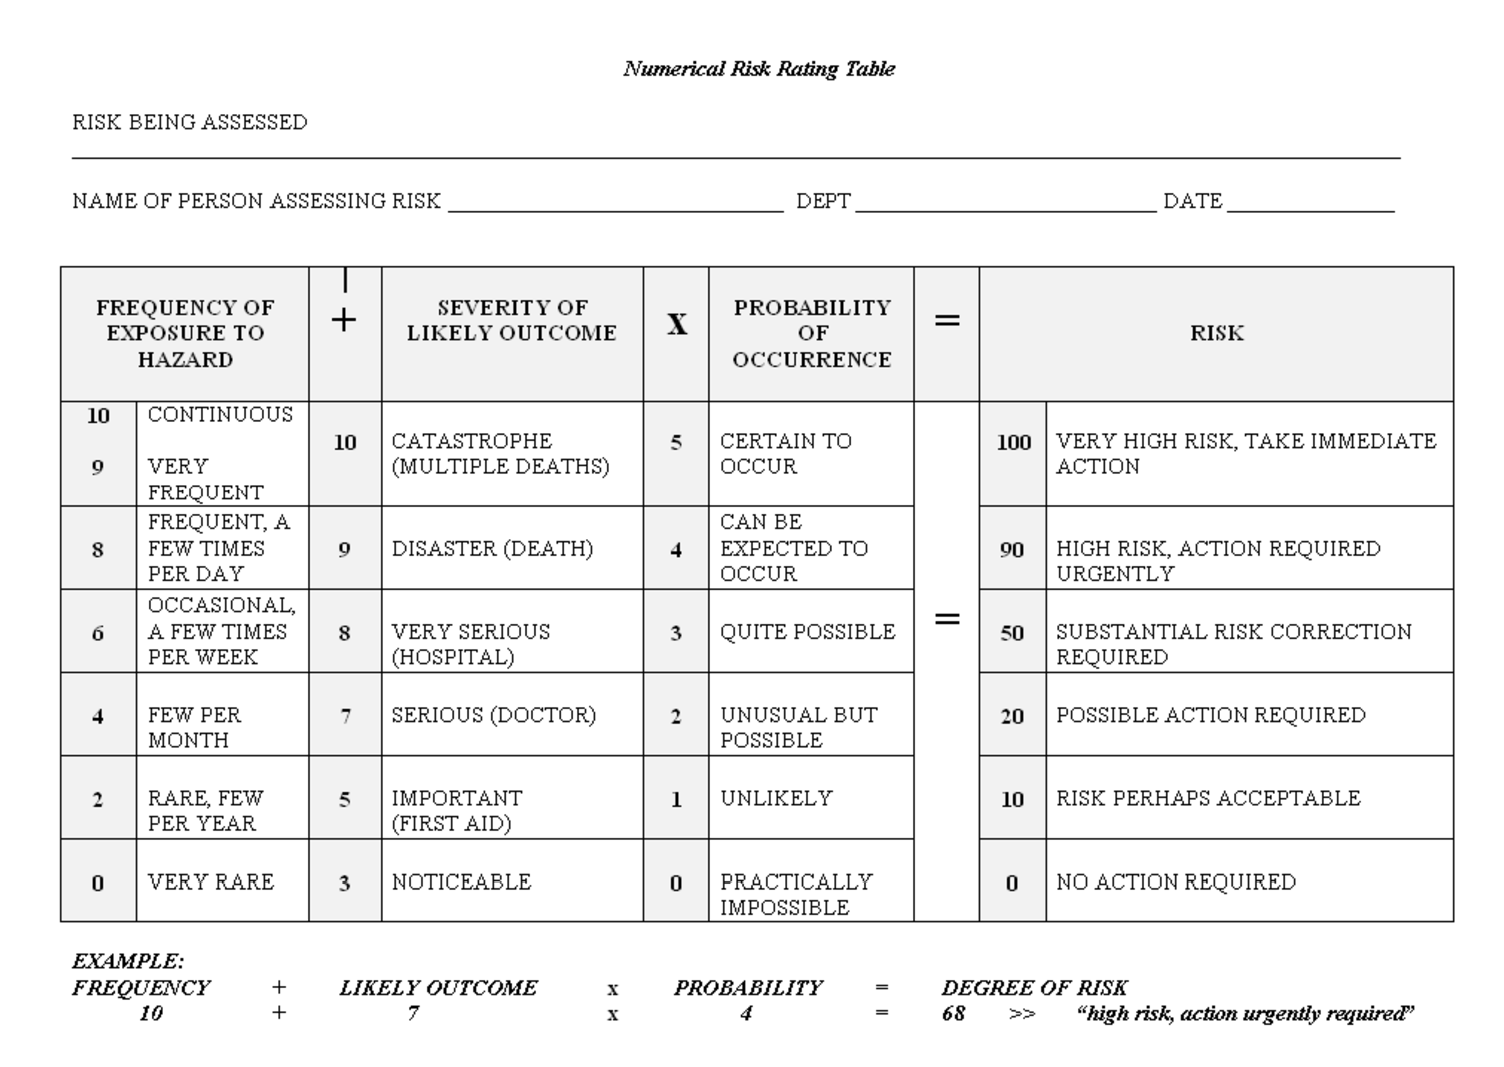
\includegraphics[angle=90,scale=0.8]{risks.pdf}

\section{Initial Bandwidth \& Power Calculations}
\label{init_calcs}
If we make a few assumptions, we can use the Friis transmission equation and the Shannon-Hartley Theorem to calculate the theoretical maximum bit rate of a radio link.

Assume:
\begin{itemize}
\item 200km Distance between TX and RX (on ground)
\item 400km radio path (via near-vertical skywave)
\item 5MHz Transmission frequency ($\lambda$ = 60m)
\item No ionospheric absorption loss (Not Realistic!)
\item Dipole antennas one each end ($G_t = G_r = 1.5$)
\item 10dB SNR required
\item -114dB\citep{ref:radio_noise} background noise at 5MHz
\end{itemize}
Using 1W transmission power, we can calculate the power at the receiving antenna:
\begin{flalign*}
P_r &= \frac{P_t G_t G_r}{(4\pi R /\lambda)^2}\\
&= \frac{1 \times 1.5 \times 1.5}{(4\pi \times 400000 / 60)^2} = 0.3206 nW = -94.94 dB\\
SNR &= 114 - 94.94 = 19.06dB = 80.54\\
\end{flalign*}
We can use the Shannon-Hartley theorem to calculate the theoretical maximum channel capacity of the link:
\[C = B \log_2 (1 + SNR) \]
Where $C$ is the channel capacity (in bits/s) and B is the signal bandwidth. Assuming Binary FSK modulation is used with a 600Hz frequency shift, we calculate the maximum channel capacity as:
\[C = 600 \log_2 (1 + 80.54) = 3809.66 \mbox{ bits/s}\]

To get a rough idea of the power usage, let us assume we are transmitting at 600 bit/s for one hour (263.67 kB of data).

The power usage of some devices that could be used are as follows:
\begin{itemize}
\item Microcontroller - 75mW in active mode \citep{ref:atmega}
\item Signal Generator - 40mW when active \citep{ref:ad9834}
\item Power Amplifier - 1W (idealised)
\end{itemize}
So under these ideal conditions, the transmitter will draw 1.115W when transmitting, which is 4014 Joules of energy for one hour of transmission. A 12V 50Ah car battery provides about 2.2 MegaJoules of energy, meaning this system could transmit for 548 hours.

\section{Project Deliverables}
\begin{table}[h!]
\begin{center}
\begin{tabular}{l|r}
\textbf{Deliverable} & \textbf{Deadline}\\
\hline
& \textbf{Semester 1}\\
Proposal Seminar & Week 3\\
Stage 1 Design Document & Thurs Week 5\\
Design Document Peer Review & Week 6\\
Progress Report & Week 11\\
Interim Performance & Week 12\\
& \textbf{Semester 2}\\
Final Project Seminar & Mid-Sem Break\\
Final Report & Week 11\\
Final Performance & Week 12\\
Project Exhibition & Week 12\\
\end{tabular}
\caption{Project Deliverables}
\label{deliverables}
\end{center}
\end{table}

\end{appendices}

\end{document}